%-------------------------------------------------------------
\documentclass[9pt, aspectratio=169]{beamer}
\usetheme{Darmstadt}
\usecolortheme{beaver}
\usepackage[french]{babel}
\usepackage{appendixnumberbeamer}
\usepackage{textpos}
\usepackage{xcolor}
\usepackage{caption}
\usepackage{subcaption}
\usepackage{array}
\usepackage[many]{tcolorbox} 
\usepackage{makecell}
\usepackage{setspace}

\usepackage{animate} % to include a GIF movie

\usepackage{stackengine}
\usepackage{scalerel}

%\usepackage[UTF8]{ctex}
%\usepackage{hyperref}
\usepackage[T1]{fontenc}
%
%\usepackage{latexsym,multicol,booktabs,calligra}
\usepackage{amsmath,amssymb} 
%\usepackage{graphicx,pstricks,stackengine}      %   
	
\usepackage{graphicx}
\usepackage[export]{adjustbox}

\usepackage{bibentry}
\nobibliography*


\captionsetup{labelformat=empty,labelsep=none,font=tiny, textfont=it}
\setbeamerfont{caption}{size=\tiny, shape=\itshape}
\setlength\belowcaptionskip{-2pt}
%\setbeamerfont{caption name}{series=\bfseries}
%\DeclareCaptionLabelFormat{mycaption}{\usebeamercolor[fg]{caption name}#1 #2. }
%\captionsetup[figure]{labelformat=mycaption, labelsep=none, labelfont=bf}

\beamertemplatenavigationsymbolsempty % remove navigation line
\setbeamertemplate{footline}[frame number] % add frame number

\definecolor{myred}{rgb}{0.8, 0.0, 0.0} % define red
\definecolor{csviolet}{rgb}{0.588, 0.008, 0.235} % define CS violet
\definecolor{iutblue}{rgb}{0.098, 0.357, 0.655} % define IUT blue
\definecolor{dgreen}{rgb}{0.,0.6,0.}

\setbeamercolor{section in head/foot}{fg=iutblue}
\setbeamercolor{subsection in head/foot}{fg=iutblue}
\setbeamercolor{frametitle}{fg=iutblue}
\setbeamercolor{itemize item}{fg=iutblue}
\setbeamercolor{itemize subitem}{fg=cyan}
\setbeamertemplate{itemize item}[circle]
\setbeamertemplate{itemize subitem}[triangle]

\setbeamercolor{section number projected}{bg=iutblue}
\setbeamertemplate{sections/subsections in toc}[circle]

% new env without headline
\makeatletter
    \newenvironment{withoutheadline}{
        \setbeamertemplate{headline}[default]
        \def\beamer@entrycode{\vspace*{-\headheight}}
    }{}
\makeatother

\makeatletter
    \newenvironment{withoutfootline}{
        \setbeamertemplate{footline}[default]
        \def\beamer@entrycode{\vspace*{-\headheight}}
    }{}
\makeatother

\addtobeamertemplate{frametitle}{}{
\begin{textblock*}{100mm}(.97\textwidth,-1cm)

\includegraphics[height=0.4cm]{fig/logos/iut.jpg}\vspace{-0.9cm}
\end{textblock*}}

%\setbeamertemplate{footline}{% 
%  \hfill% 
%  \usebeamercolor[fg]{page number in head/foot}% 
%  \usebeamerfont{page number in head/foot}% 
%  \insertframenumber%
%  %\,/\,\inserttotalframenumber
%  \kern1em\vskip2pt% 
%}

\definecolor{crimson}{rgb}{0.86, 0.08, 0.24}
\definecolor{myGreen}{rgb}{0.2, 0.71, 0.2}
\definecolor{babyblue}{rgb}{0.54, 0.81, 0.94}
\definecolor{tabblue}{RGB}{31, 119, 180}


\newtcolorbox{myblockred}[1]{%
    tikznode boxed title,
    enhanced,
    arc=3mm,
    interior style={white},
    attach boxed title to top center= {yshift=-\tcboxedtitleheight/2},
    fonttitle=\bfseries,
    colbacktitle=white,coltitle=crimson,
    boxed title style={size=normal,colframe=white,boxrule=0pt},
    before upper={\parindent15pt},
    title={#1}
}

\newtcolorbox{myblockgreen}[1]{%
    tikznode boxed title,
    enhanced,
    arc=3mm,
    interior style={white},
    attach boxed title to top center= {yshift=-\tcboxedtitleheight/2},
    fonttitle=\bfseries,
    colbacktitle=white,coltitle=myGreen,
    boxed title style={size=normal,colframe=white,boxrule=0pt},
    before upper={\parindent15pt},
    title={#1}
}

\newtcolorbox{myblockblue}[1]{%
    tikznode boxed title,
    enhanced,
    arc=3mm,
    interior style={white},
    attach boxed title to top center= {yshift=-\tcboxedtitleheight/2},
    fonttitle=\bfseries,
    colbacktitle=white,coltitle=babyblue,
    boxed title style={size=normal,colframe=white,boxrule=0pt},
    before upper={\parindent15pt},
    title={#1}
}
%% COMMAND
\newcommand{\dbspl}{dB$_{\text{SPL}}$}
\newcommand{\dms}{$\Delta$MS}
\newcommand{\dsnr}{$\Delta$SNR}
\newcommand{\DSNR}{\Delta \text{SNR}}
\newcommand{\vect}[1]{\boldsymbol{#1}}
\newcommand{\thc}{^\text{th}}
%
\newcommand{\wv}{\boldsymbol{w}}
\newcommand{\xv}{\boldsymbol{x}}
\newcommand{\hv}{\boldsymbol{h}}
\newcommand{\nv}{\boldsymbol{n}}
\newcommand{\gv}{\boldsymbol{g}}
\newcommand{\qv}{\boldsymbol{q}}
%
\newcommand{\sv}{\boldsymbol{s}}
\newcommand{\Hm}{\boldsymbol{H}}
\newcommand{\Gm}{\boldsymbol{G}}
%
\newcommand{\snrout}{\rho_{\text{out}}}
\newcommand{\esp}[1]{\mathbb{E}\left[#1\right]}
\newcommand{\m}[1]{\mathcal{M}_#1}

\newcommand{\Le}{\text{L}}
\newcommand{\Rea}{\text{R}}

\newcommand{\kl}{{k, \ell}}
\newcommand{\kpl}{{\kappa, \ell}}
\newcommand{\argmin}[2]{\underset{#1}{\text{argmin}} \left\lbrace #2 \right\rbrace}

\newcommand{\xmark}{\textcolor{red}{\ding{55}}}

\newcommand{\tildep}{{\tilde{\text{p}}}}

\newcommand\dangersign[1][2ex]{%
  \renewcommand\stacktype{L}%
  \scaleto{\stackon[1.3pt]{\color{red}$\triangle$}{\tiny\bfseries !}}{#1}%
}

%—-------------------------------------------------------------
\begin{document}

\begin{withoutheadline}
\begin{withoutfootline}
\begin{frame}
	% LOGO 
	\begin{figure}
	\begin{subfigure}{.45\linewidth}
	\begin{flushleft}
		\hspace{-0.5cm}
		
\includegraphics[width=0.2\linewidth]{fig/logos/iut.jpg}
	\end{flushleft}
	\end{subfigure}
	\begin{subfigure}{.45\linewidth}
	\begin{flushright}
		
\includegraphics[width=0.5\linewidth]{fig/logos/LTSI.png}
	\end{flushright}
	\end{subfigure}
	\end{figure}
	\vspace{0.5cm}
	% Title
	\textbf{\large Codage audio}

	\vspace{1.4cm}
	\footnotesize Adrien Llave
	\vspace{0.2cm}

	\footnotesize 14 novembre 2023
\end{frame}
\end{withoutfootline}
\end{withoutheadline}

% --- TOC ------------------------------------------------------------------
\begin{withoutheadline}
\begin{frame}{Sommaire}
	\tableofcontents[sectionstyle=show,subsectionstyle=show/shaded/hide,subsubsectionstyle=show/shaded/hide]
\end{frame}
\end{withoutheadline}

\begin{frame}{Objectifs} %-----------------------------------------------------
\begin{center}

    \begin{itemize}
        \item Démystifier le traitement du signal (et la théorie de l'information)
        \item Donner quelques intuitions sur la compression de données
        \item Donner un peu de culture technique
    \end{itemize}
\end{center}
\end{frame}

\begin{frame}{D'où je parle} %-----------------------------------------------------
\begin{center}

    \begin{itemize}
        \item 2010 - 2012 : IUT GEII
        \item 2012 - 2015 : Master métiers du son à l'ENS Louis-Lumière
        \item 2015 - 2016 : Master traitement du signal à Grenoble-INP Phelma
        \item 2017 - 2022 : Doctorat traitement du signal à CentraleSupélec
        \item 2022 - 2023 : Chercheur à Orange
        \item 		 2023 : Enseignement à l'IUT, recherche au LTSI
        \item 2024 -      : Chercheur à Orange
    \end{itemize}
\end{center}
\end{frame}


%==================================================================================================
%==================================================================================================
%==================================================================================================	
\section{Traitement du signal}

\begin{frame}{} %-----------------------------------------------------
\begin{center}
\Huge \insertsection
\end{center}
\end{frame}

\begin{frame}{\og Traitement du signal \fg{} ???} %-----------------------------------------------------
Pensons à une science... \pause la \textbf{biologie} :
\pause
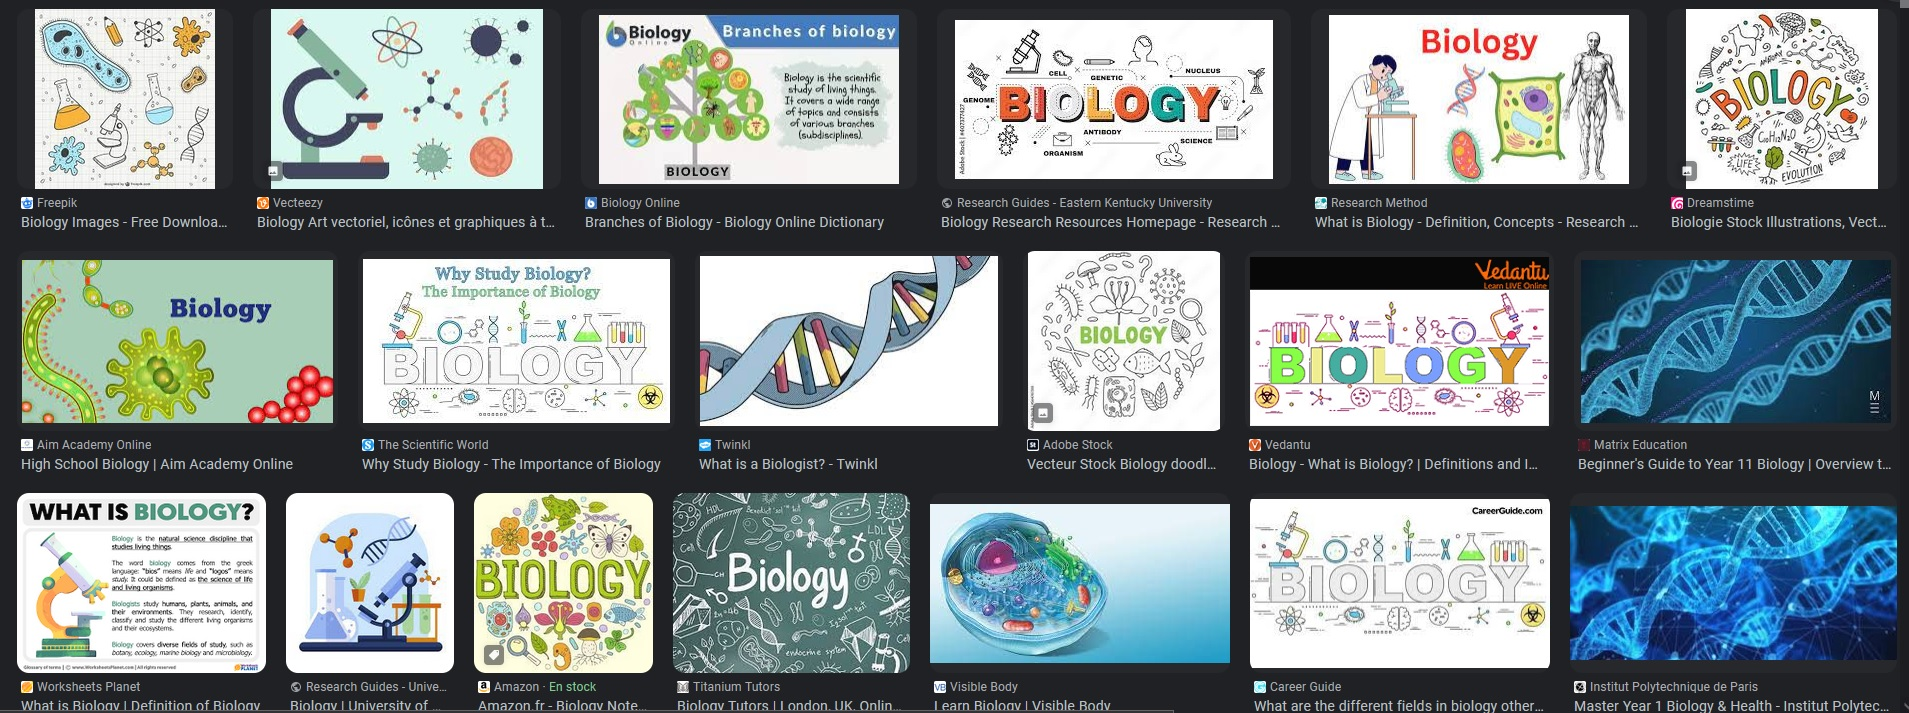
\includegraphics[width=\textwidth]{fig/search_results_biology.jpg}
\pause
\begin{itemize}
    \item la biologie est faite par les... biologistes :)
    \item mots-clés : \textbf{ADN, cellule, microscope, organisme, vivant}...
\end{itemize}

\end{frame}

\begin{frame}{\og Traitement du signal \fg{} ???} %-----------------------------------------------------

Et maintenant le \textbf{traitement du signal} :
\pause
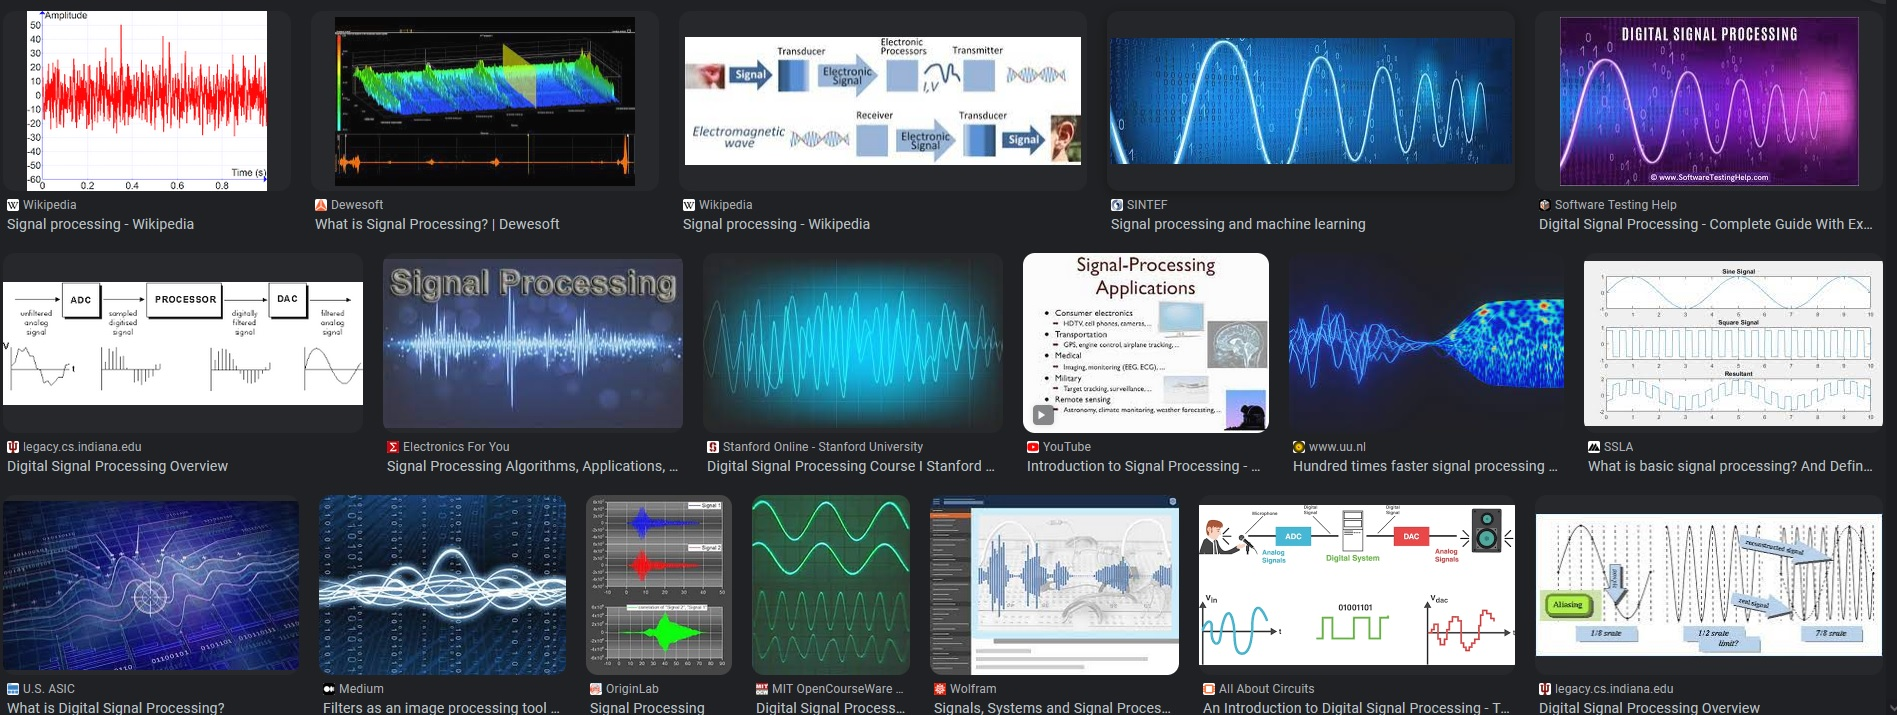
\includegraphics[width=\textwidth]{fig/search_results_signal_proc.jpg}
\pause
\begin{itemize}
    \item le traitement du signal est fait par les... ? \pause traiteur-euses ? \pause sémaphoricien-nes ?
    \pause
    \item mots-clés : \textbf{sinusoïde, quantification, binaire}. C'est tout ?  :(
\end{itemize}

\end{frame}

\begin{frame}{Quelques définitions : \og traitement du signal \fg{}} %-----------------------------------------------------
\begin{columns}
   \begin{column}{0.4\textwidth}
        \begin{myblockred}{\textbf{traitement}}
        \begin{itemize}
            \item analyse
            \item communication (stockage)
            \item synthèse
        \end{itemize}
        \end{myblockred}
        
   \end{column}
   \begin{column}{0.59\textwidth}
		\begin{myblockred}{\textbf{signal}}
        mesure physique contenant de l'\textbf{information}
        \end{myblockred}
   \end{column}
\end{columns}

\vspace{1cm}
\textbf{information} : ce qui aide à la \textbf{décision}

\end{frame}


\begin{frame}{Quelques définitions : \og Décision \fg{}} %-----------------------------------------------------

\begin{itemize}
    \item \textbf{binaire} : gauche/droite, thé/café, fromage/dessert, vrai/faux, ...
    \item \textbf{discrète} (discontinue) : "quel étage ?", "quel âge ?", ... \\
    $\rightarrow$ décisions binaires en cascade
    \item \textbf{continue} : "quelle température ?" \\
    $\rightarrow$ seuil de perception $\rightarrow$ discontinue
\end{itemize}
\end{frame}

\begin{frame}{Fromage ou dessert ?} %-----------------------------------------------------
\begin{columns}
   \begin{column}{0.6\textwidth}
        Le plus simple : un arbre de décision à deux branches

        $\rightarrow$ notation binaire ! 0 ou 1
        
   \end{column}
   \begin{column}{0.39\textwidth}
		
\includegraphics[width=\textwidth]{fig/choice_left_right.jpg}
   \end{column}
\end{columns}
\end{frame}

\begin{frame}{Itinéraire} %-----------------------------------------------------
\begin{columns}
   \begin{column}{0.6\textwidth}
		Guidage itinéraire : droite/gauche/tout-droit/STOP

        \begin{table}[]
            \begin{tabular}{l|c|c}
            \textbf{Décision}    & \textbf{1er bit} & \textbf{2eme bit} \\
            \hline
             Droite     & 0 & 0  \\
             Gauche     & 1 & 0 \\
             Tout-droit & 0 & 1 \\
             STOP       & 1 & 1\\
        \end{tabular}
        \end{table}

        droite-droite-gauche-gauche-STOP = 00 00 10 10 11
        
        $\rightarrow$ 10 bits
        
   \end{column}
   \begin{column}{0.39\textwidth}
		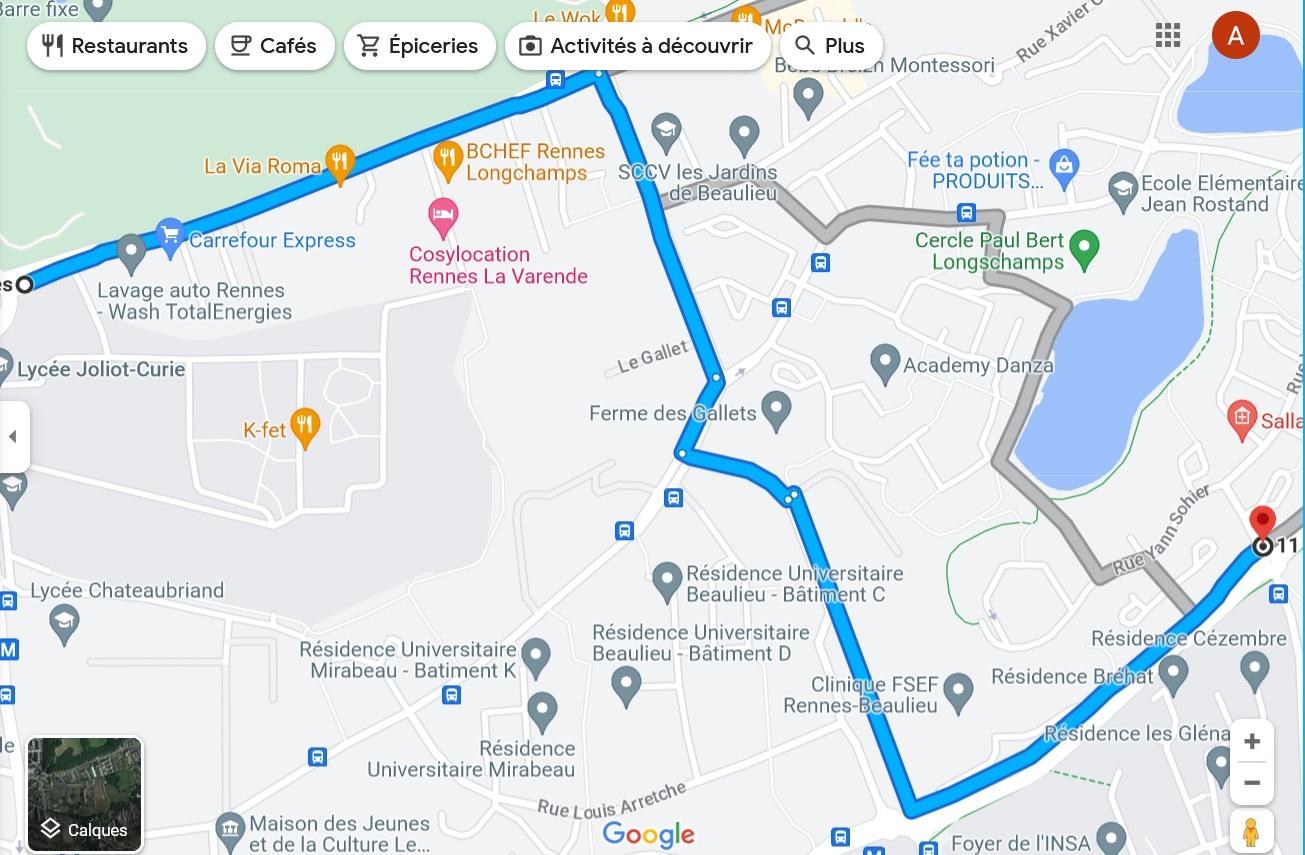
\includegraphics[width=\textwidth]{fig/maps_iut_gayeulles.jpg}
   \end{column}
\end{columns}
\end{frame}

\begin{frame}{Qui est-ce ?} %-----------------------------------------------------
\begin{columns}
   \begin{column}{0.55\textwidth}
    Règle du jeu :
    \begin{itemize}
        \item poser une question fermée (oui/non) à chaque tour
        \item trouver la personne cachée en un \textbf{minimum} de tour
    \end{itemize}
    
    Exemples de questions :
    \begin{itemize}
        \item blond ?
        \item homme/femme ?
        \item lunette ?
        \item ...
    \end{itemize}
        
   \end{column}
   \begin{column}{0.45\textwidth}
		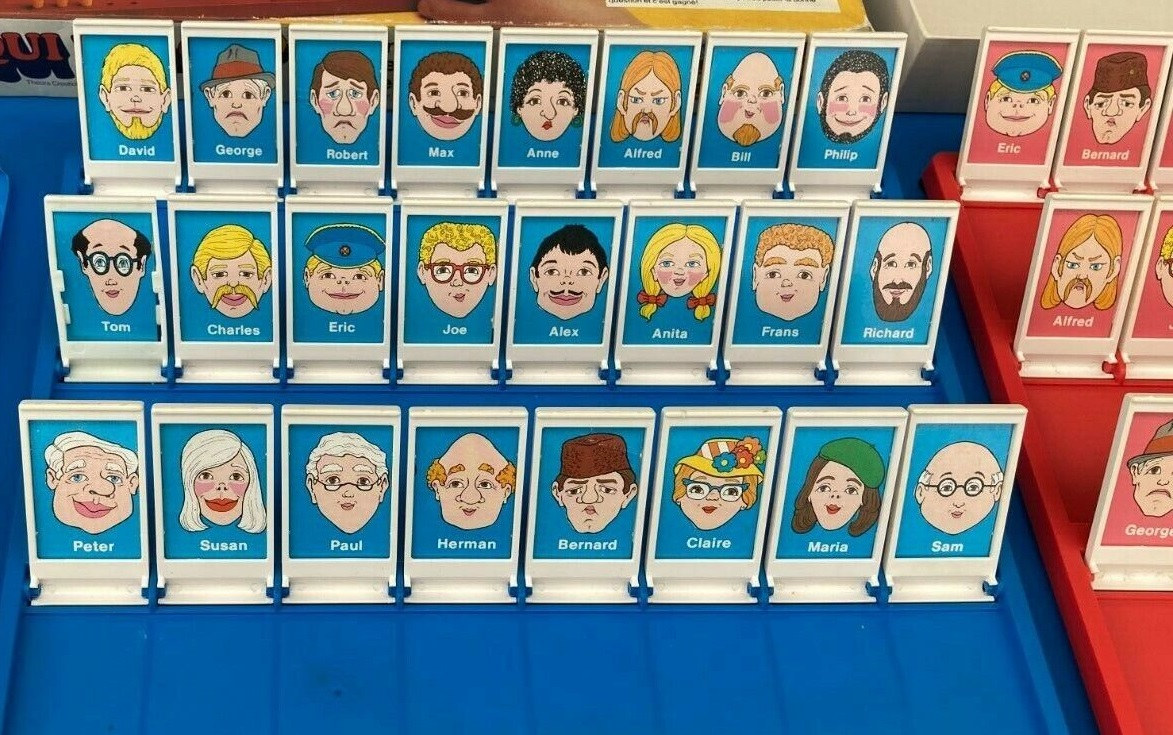
\includegraphics[width=\textwidth]{fig/jeuquiestce.jpg}
   \end{column}
\end{columns}
\end{frame}

\begin{frame}{Température} %-----------------------------------------------------
\begin{columns}
   \begin{column}{0.55\textwidth}
        Effet de seuil de perception
   \end{column}
   \begin{column}{0.45\textwidth}
		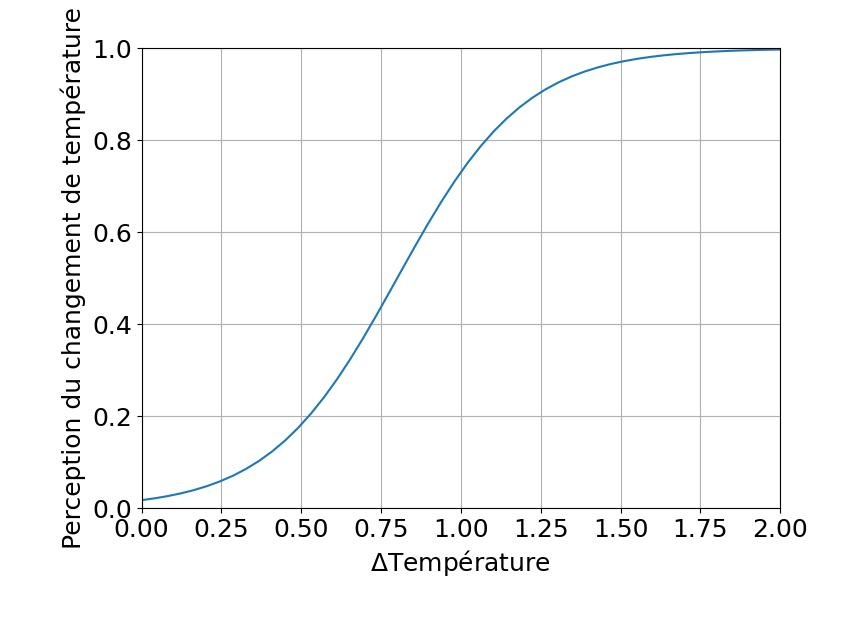
\includegraphics[width=\textwidth]{fig/sigmoid_temperature.jpg}
   \end{column}
\end{columns}
\end{frame}


%==================================================================================================
%==================================================================================================
%==================================================================================================	
\section{Compression - intro}

\begin{frame}{} %-----------------------------------------------------
\begin{center}
\Huge \insertsection
\end{center}
\end{frame}
%==================================================================================================	

\begin{frame}{Quelques ordres de grandeur...} %-----------------------------------------------------
\begin{columns}
   \begin{column}{0.6\textwidth}
   \begin{itemize}
       \item Exemple : itinéraire IUT $\rightarrow$ Parc des Gayeulles
       \item Capture d'écran :
            \begin{itemize}
            \item \textbf{bitmap 24 bits} : 3270 ko = 26'160'000 bits !
            \item \textbf{png} (sans perte) : 572 ko = 4'576'000 bits‬
            \item \textbf{jpg} (avec perte) : 297 ko = 2'376'000 bits
            \end{itemize}
        \item \textbf{old school} : "droite/gauche/tout-droit/STOP" :
            \begin{itemize}
            \item droite-droite-gauche-gauche-STOP = 10 bits
            \end{itemize}
   \end{itemize}
		
   \end{column}
   \begin{column}{0.39\textwidth}
		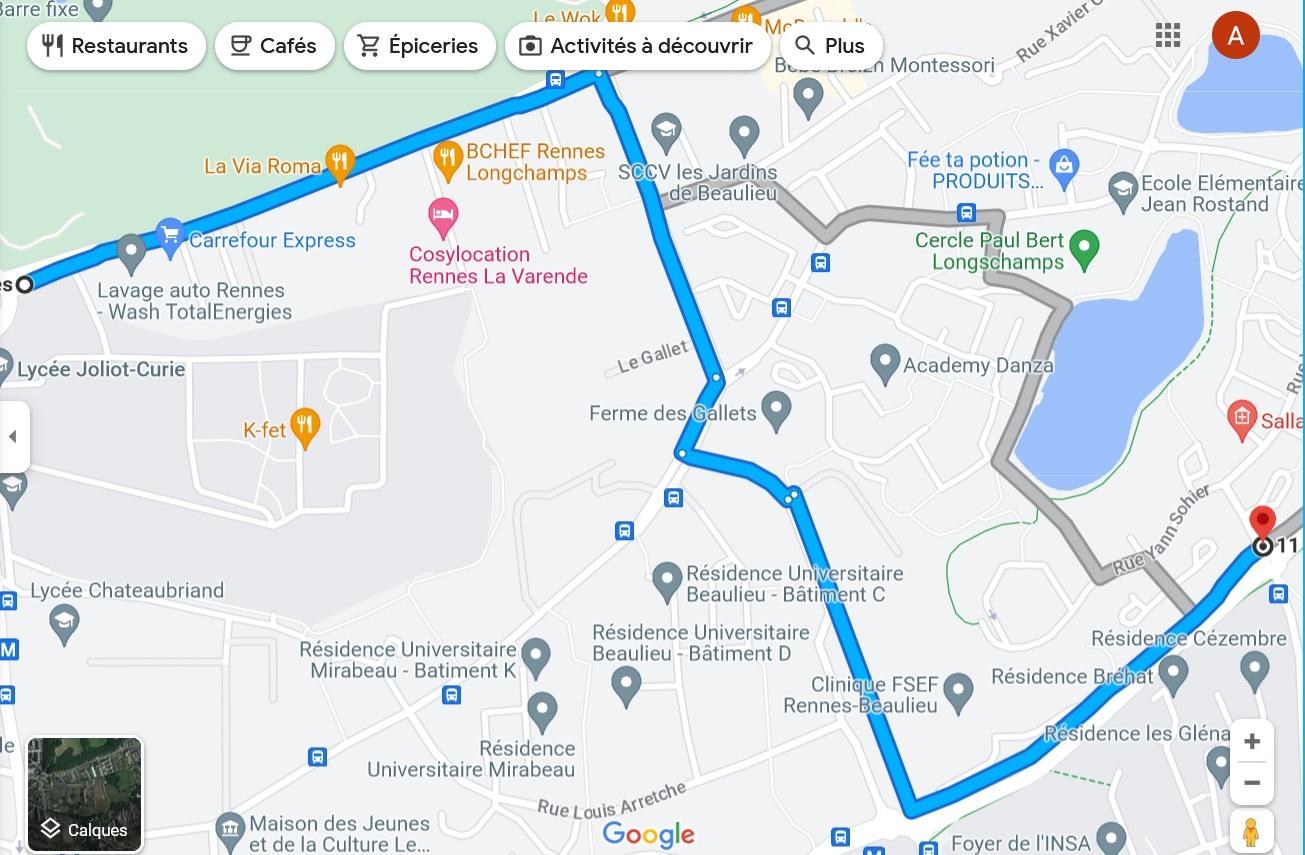
\includegraphics[width=\textwidth]{fig/maps_iut_gayeulles.jpg}
   \end{column}
\end{columns}
\end{frame}

\begin{frame}{\og Codage \fg{} ?} %-----------------------------------------------------

\begin{myblockblue}{Exemples de \url{https://fr.wikipedia.org/wiki/Codage}}
	  \begin{itemize}
     \item Le codage de l'information désigne les moyens de formaliser l'information.
     \item Un codage des caractères définit une manière de représenter les caractères (lettres, chiffres, symboles) dans un système informatique.
    \item En psychologie cognitive de la mémoire, le codage est le processus par lequel une information est mise en mémoire.
    \item Le codage de source, qui permet de faire de la compression de données.
    \item le codage de canal, qui permet une représentation des données de façon à être résistant aux erreurs de transmission.
 \end{itemize}
\end{myblockblue}
    
\end{frame}

%==================================================================================================	
%==================================================================================================	
%==================================================================================================	
\section{Compression sans pertes}

\begin{frame}{} %-----------------------------------------------------
\begin{center}
\Huge \insertsection
\end{center}
\end{frame}

\begin{frame}{Itinéraire} %-----------------------------------------------------
\begin{columns}
   \begin{column}{0.6\textwidth}
        Devine un nombre (réponse + ou -) : navigation dans un arbre
	
        \begin{itemize}
        \item meilleure stratégie avec a priori équiprobable
	    \item meilleure stratégie si 0 la moitié du temps
        \end{itemize}
        
   \end{column}
   \begin{column}{0.39\textwidth}
		
\includegraphics[width=\textwidth]{fig/choice_left_right.jpg}
   \end{column}
\end{columns}
\end{frame}

\begin{frame}{Quantité d'information} %-----------------------------------------------------

On note $H(X)$ la quantité d'information contenue dans un message binaire $X$ :
\begin{equation*}
    H(X) = p \log_2\left(\frac{1}{p}\right) + (1-p) \log_2\left(\frac{1}{1-p}\right)
\end{equation*}

\animategraphics[loop,controls,width=.5\textwidth]{10}{fig/binary_entropy/binary_entropy-}{0}{49}

\end{frame}

\begin{frame}{Texte : redondance des caractères} %-----------------------------------------------------
Codage de texte = \og Qui est-ce ? \fg{}
\begin{columns}
   \begin{column}{0.6\textwidth}
        
        \only<1>{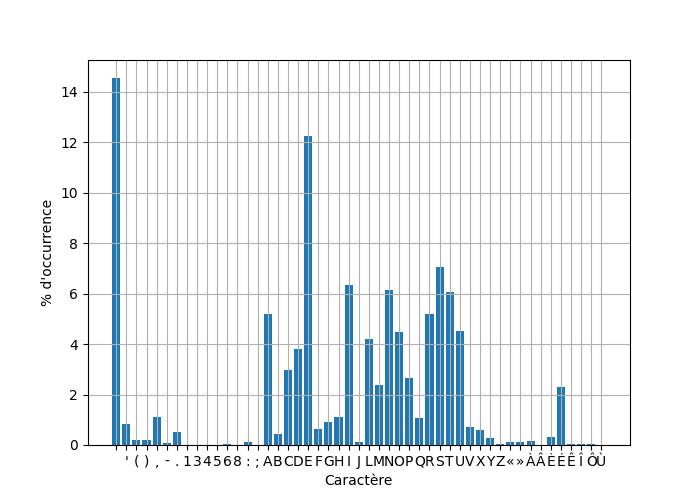
\includegraphics[width=\textwidth]{fig/text_hist_raw.jpeg}}
        \only<2>{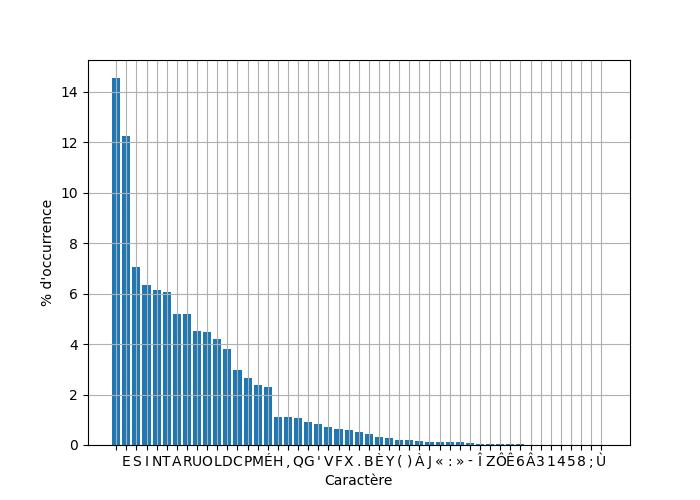
\includegraphics[width=\textwidth]{fig/text_hist_sort.jpeg}}
        
   \end{column}
   \begin{column}{0.39\textwidth}
		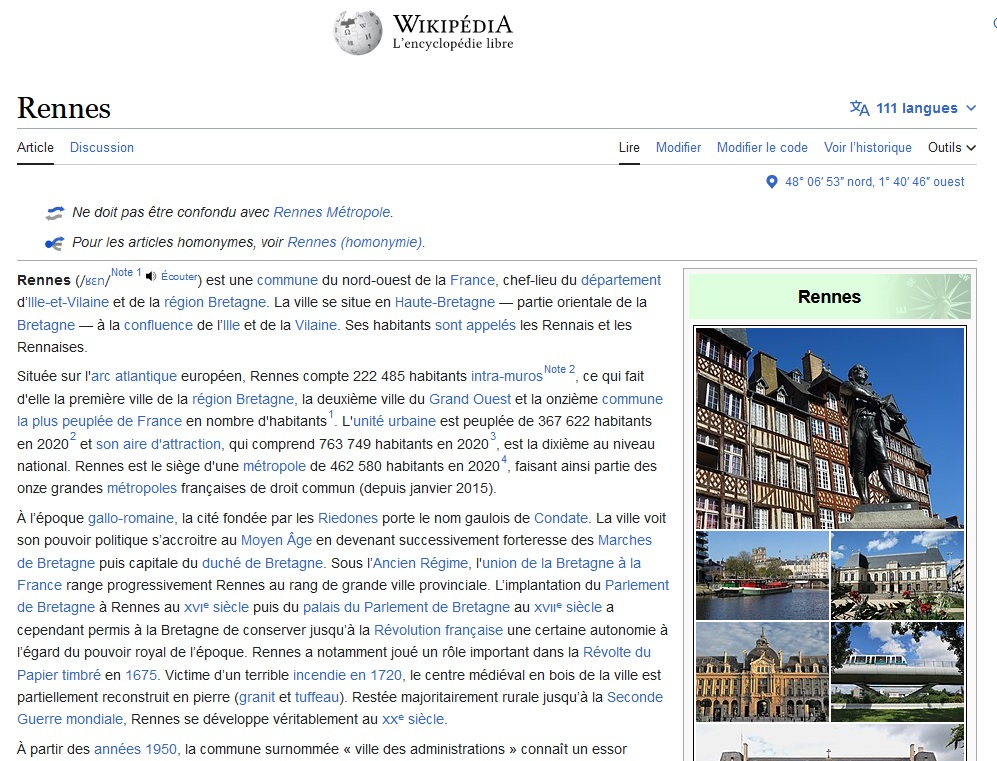
\includegraphics[width=\textwidth]{fig/wiki_rennes.jpg}
   \end{column}
\end{columns}
\end{frame}

\begin{frame}{Applications} %-----------------------------------------------------
\begin{columns}
   \begin{column}{0.6\textwidth}
		Codage entropique :
        \begin{itemize}
            \item Image : PNG (Portable Network Graphics)
            \item Audio : FLAC (Free Lossless Audio Codec)
            \item tout type de fichier : ZIP, RAR, ...
        \end{itemize}
        
   \end{column}
   \begin{column}{0.39\textwidth}
		
   \end{column}
\end{columns}
\end{frame}

\begin{frame}{Redondance temporelle} %-----------------------------------------------------

\begin{columns}
   \begin{column}{0.6\textwidth}

        Problème : considérons le message \textbf{"ABCDABCDABCDAB"}. Quelle sera la lettre suivante ?
        \begin{itemize}
            \item "A", "B", "C" et "D" sont équiproblables
            \item Le message n'est pas "redondant" au sens de l'entropie de Shannon
            \item Pourtant, on devine que la lettre suivante sera "C"
        
        \end{itemize}
        
   \end{column}
   \begin{column}{0.39\textwidth}
		
   \end{column}
\end{columns}
\end{frame}


\begin{frame}{Quantifier la redondance temporelle} %-----------------------------------------------------

\begin{columns}
   \begin{column}{0.6\textwidth}


        \begin{itemize}
            \item Pour les redondances de symbole : entropie de Shannon
            \item Pour les redondances temporelle : entropie de Wiener
            \begin{equation*}
            	\xi = \frac{\left(\Pi\limits_{i=1}^N P_i \right)^\frac{1}{N}}{\frac{1}{N}\sum\limits_{i=1}^N P_i}
            \end{equation*}
            avec $P_i$ la puissance du spectre à la fréquence $i$.
            \item $\xi \in [0, 1]$ quantifie l'aplatissement du spectre
        
        \end{itemize}
        
   \end{column}
   \begin{column}{0.39\textwidth}
		
   \end{column}
\end{columns}
\end{frame}

\begin{frame}{Codage par prédiction linéaire} %-----------------------------------------------------

\begin{columns}
   \begin{column}{0.6\textwidth}
		
		Idée :
        \begin{itemize}
	        \item Je peux prédire l'échantillon présent à partir du passé: 
	        \begin{equation*}
	       		x_n = \underbrace{f(x_{n-1}, x_{n-2}, ..., x_{n-P})}_{\hat{x}_n}  + \epsilon_n
	        \end{equation*}
	        \item Quelle approximation pour $f(.)$ ? $\rightarrow$ combinaison linéaire
	        \begin{equation*}
	        	\hat{x}_n = \sum\limits_{i=1}^N a_i . x_{n-i}
	        \end{equation*}
            \item Décorréler le signal\\
            $\rightarrow$ trouver un filtre \og blanchisseur \fg{}
            \item le signal \og blanchi \fg{} est moins puissant que l'original \\
            $\rightarrow$ moins de bits pour une même précision
        \end{itemize}
        
   \end{column}
   \begin{column}{0.39\textwidth}
		
   \end{column}
\end{columns}
\end{frame}

\begin{frame}{Codage par prédiction linéaire - exemple} %-----------------------------------------------------


\begin{columns}
   \begin{column}{0.2\textwidth}
	
        \tiny Idée :
        \begin{itemize}
            \item Décorréler le signal\\
            $\rightarrow$ trouver un filtre \og blanchisseur \fg{}
            \item le signal \og blanchi \fg{} est moins puissant que l'original \\
            $\rightarrow$ moins de bits pour une même précision
        \end{itemize}
        
   \end{column}
   \begin{column}{0.8\textwidth}
		\animategraphics[loop,controls,width=\textwidth]{10}{fig/lpc_speech_anime/lpc_speech_}{0}{99}

   \end{column}
\end{columns}


\end{frame}

\begin{frame}{Applications} %-----------------------------------------------------
\begin{columns}
   \begin{column}{0.6\textwidth}
		Codage entropique :
        \begin{itemize}
            \item Image : PNG (Portable Network Graphics)
            \item Audio : FLAC (Free Lossless Audio Codec)
            \item tout type de fichier : ZIP, RAR, ...
        \end{itemize}
        
   \end{column}
   \begin{column}{0.39\textwidth}
		
   \end{column}
\end{columns}
\end{frame}


%==================================================================================================	
%==================================================================================================	
%==================================================================================================	
\section{Compression avec pertes}
\begin{frame}{} %-----------------------------------------------------
\begin{center}
\Huge \insertsection
\end{center}
\end{frame}

\begin{frame}{Quantification} %-----------------------------------------------------
\begin{columns}
   \begin{column}{0.6\textwidth}
		
   \end{column}
   \begin{column}{0.39\textwidth}
		
   \end{column}
\end{columns}
\end{frame}

\begin{frame}{Codage par transformée : changer de point de vue} %-----------------------------------------------------
\begin{columns}
   \begin{column}{0.6\textwidth}
		La meilleure stratégie ? 
  
        
        
   \end{column}
   \begin{column}{0.39\textwidth}
		
   \end{column}
\end{columns}
\end{frame}

\begin{frame}{Codage par transformée : changer de point de vue} %-----------------------------------------------------


\only<1>{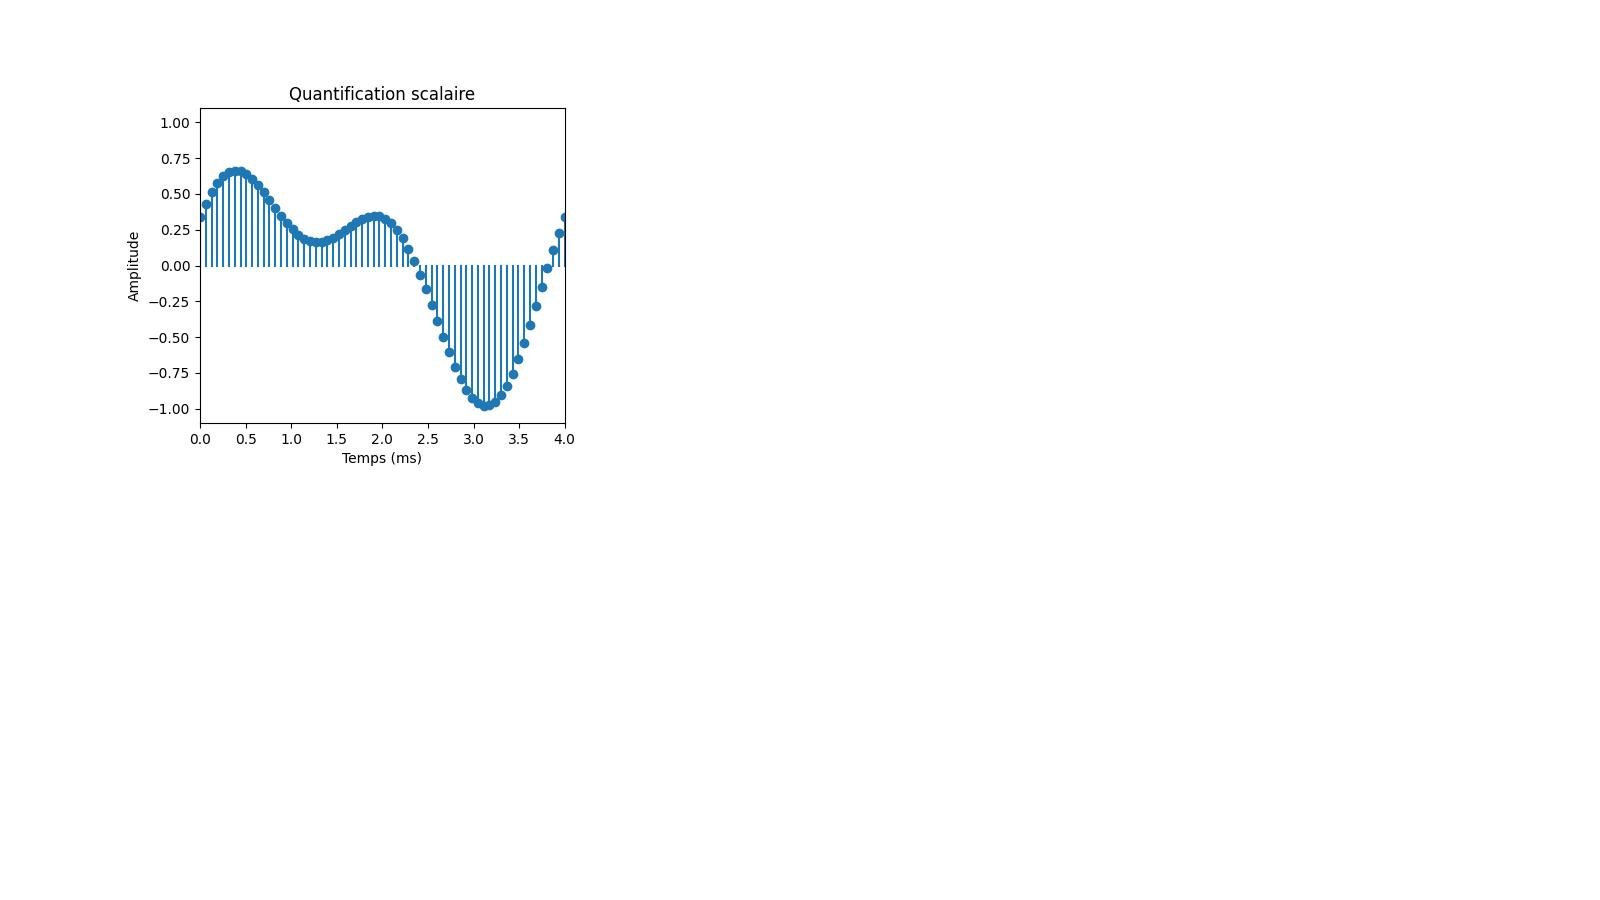
\includegraphics[width=.8\textwidth]{fig/tc_example_1.jpg}}
\only<2>{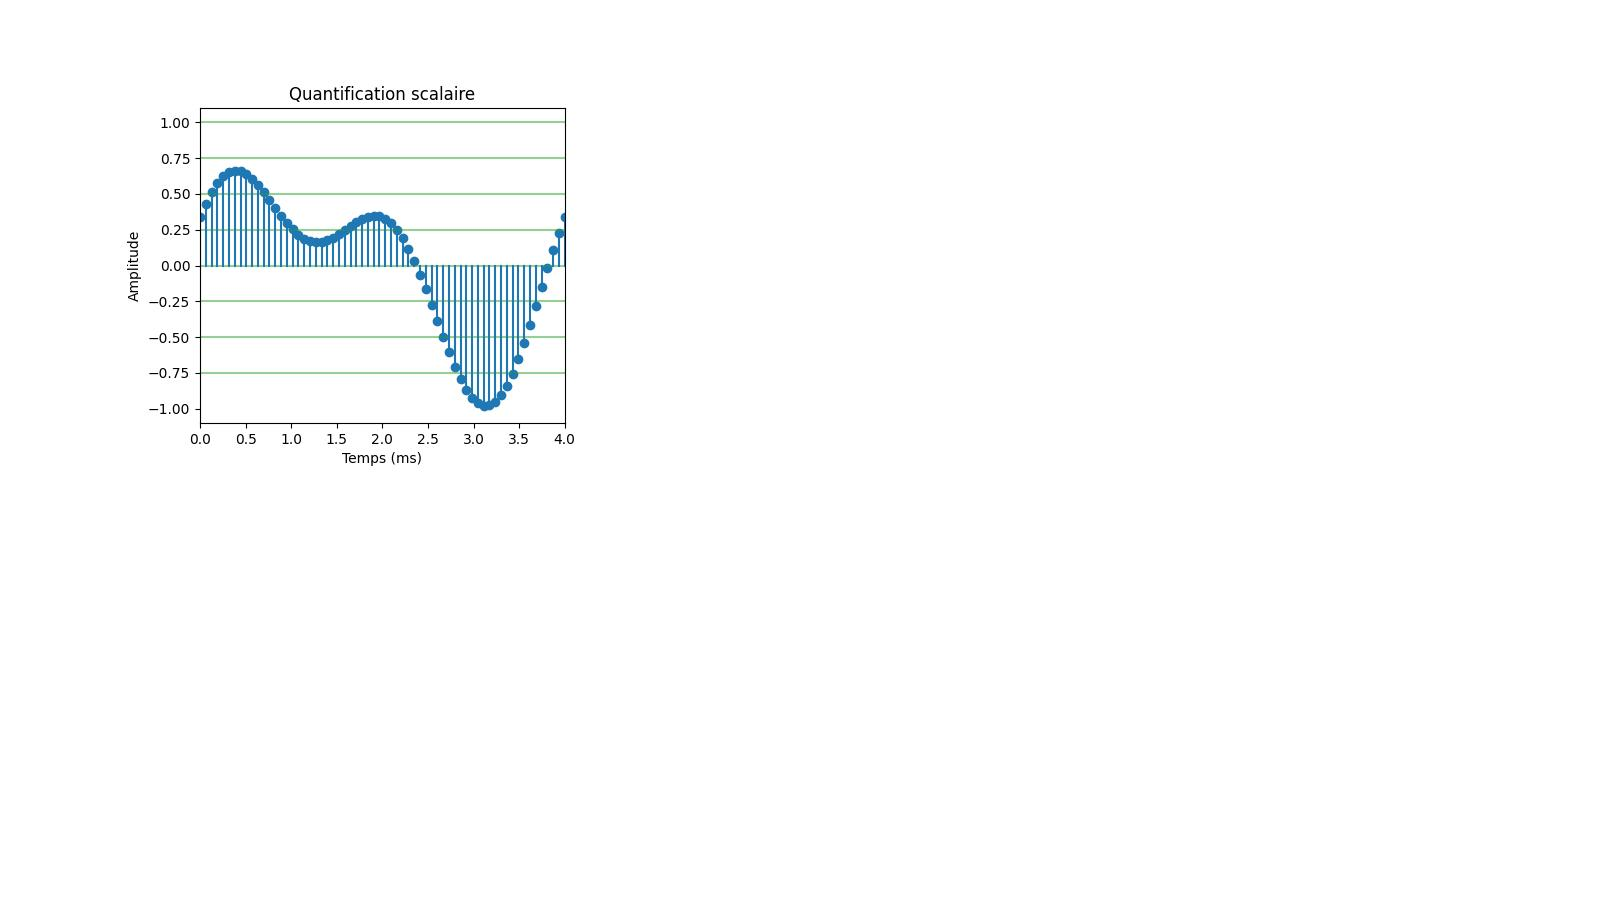
\includegraphics[width=.8\textwidth]{fig/tc_example_2.jpg}}
\only<3>{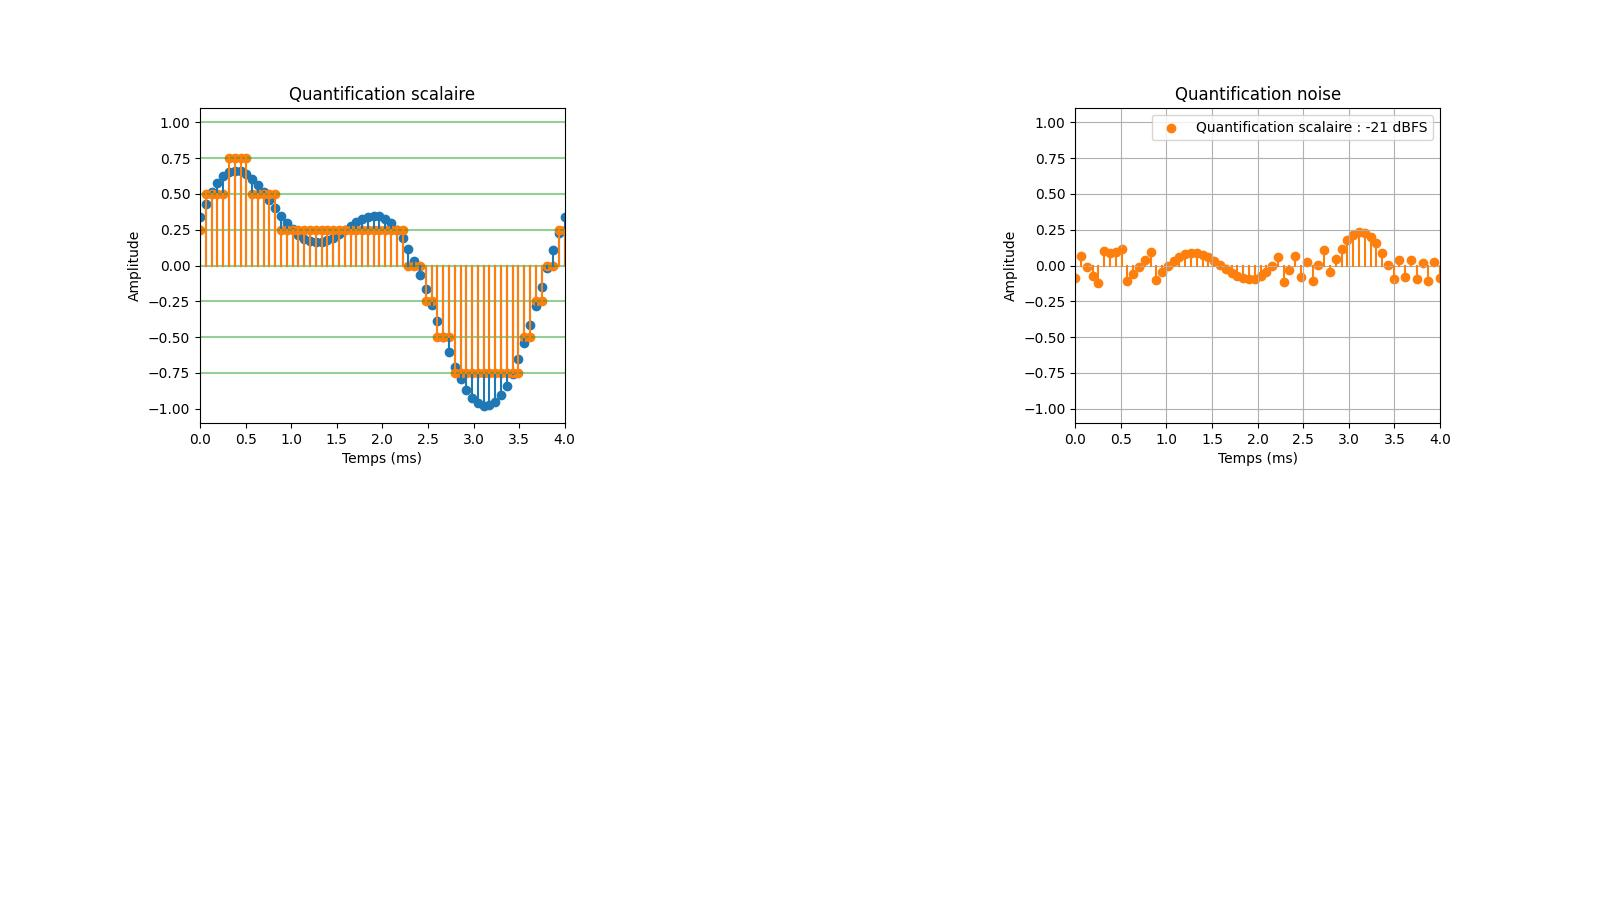
\includegraphics[width=.8\textwidth]{fig/tc_example_3.jpg}}
\only<4>{\animategraphics[loop,controls,width=.8\textwidth]{1}{fig/tc_frame_anime/tc_frame_}{1}{31}}
\only<5>{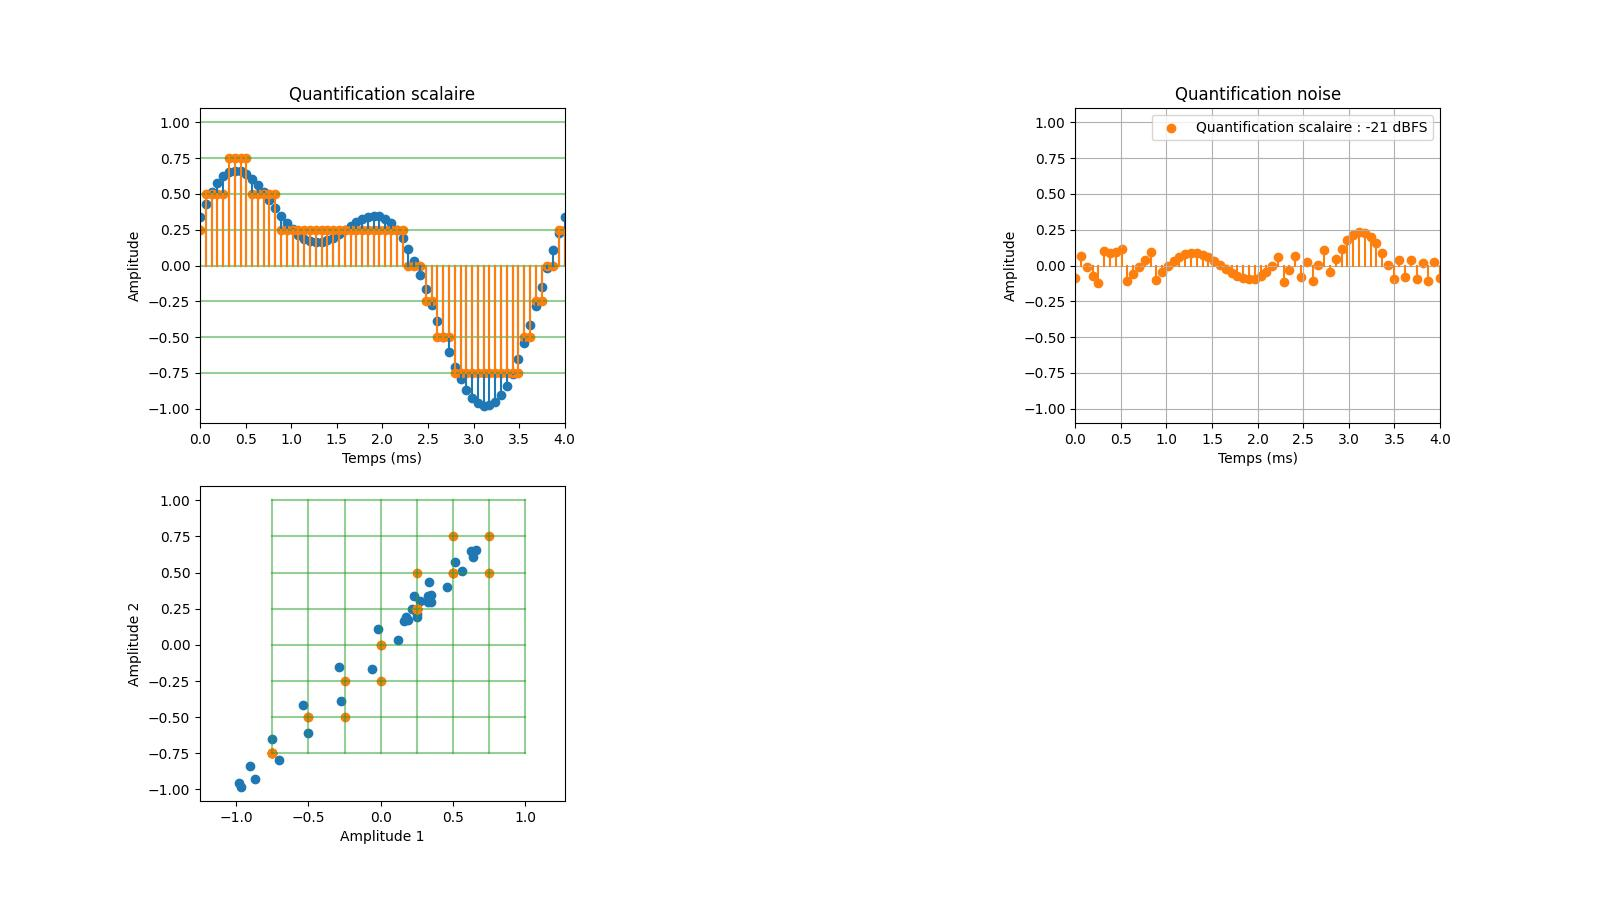
\includegraphics[width=.8\textwidth]{fig/tc_example_4.jpg}}
\only<6>{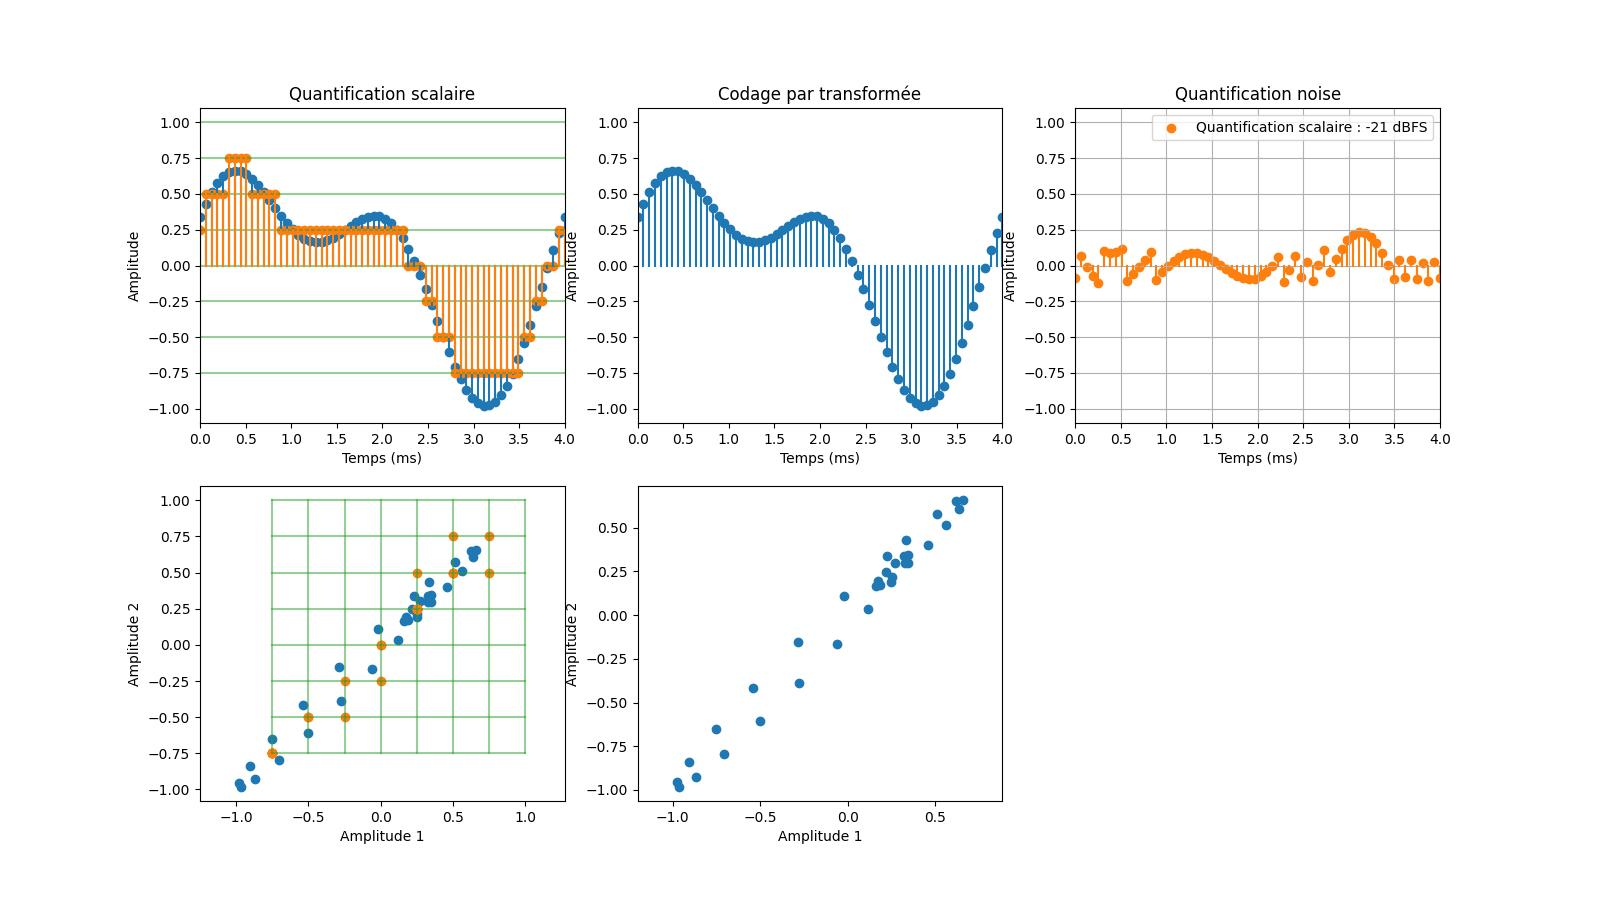
\includegraphics[width=.8\textwidth]{fig/tc_example_5.jpg}}
\only<7>{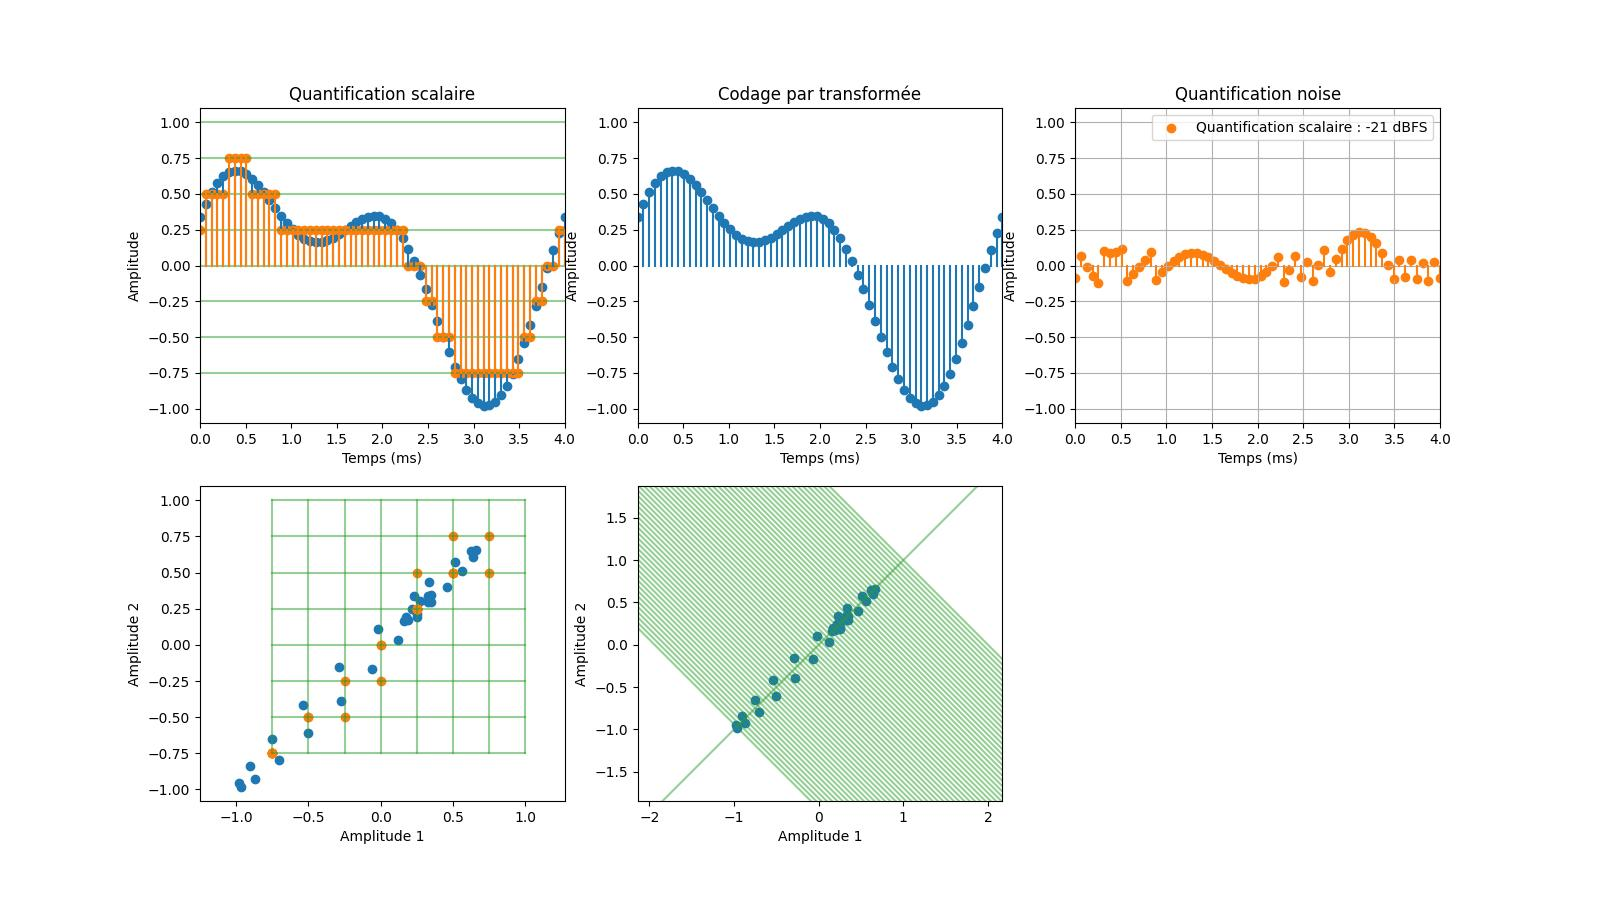
\includegraphics[width=.8\textwidth]{fig/tc_example_6.jpg}}
\only<8>{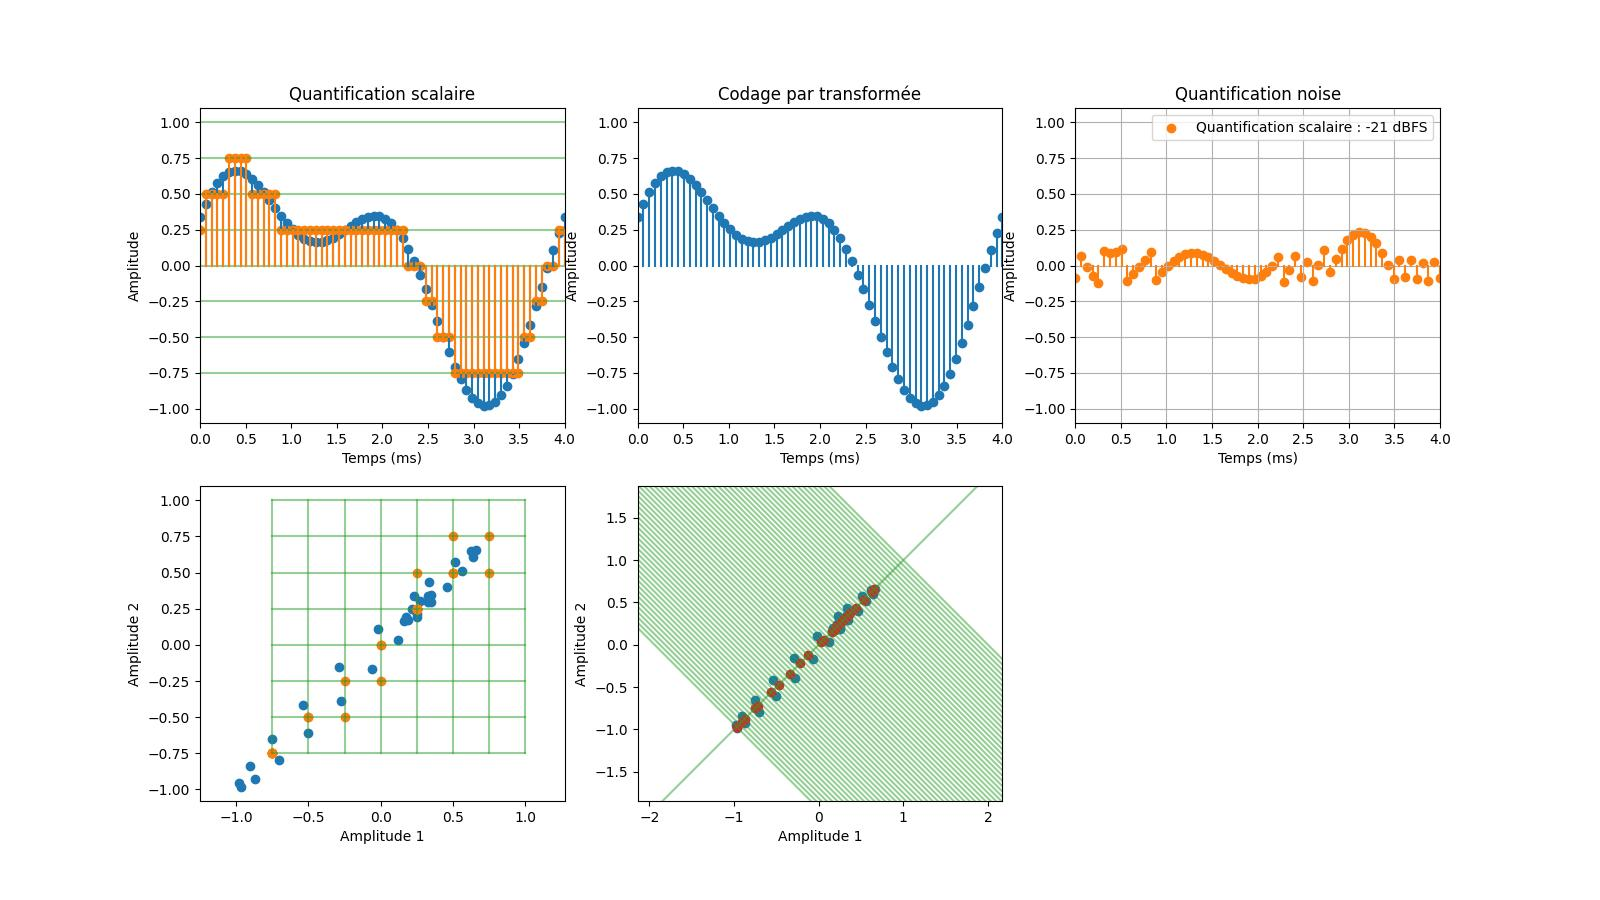
\includegraphics[width=.8\textwidth]{fig/tc_example_7.jpg}}
\only<9>{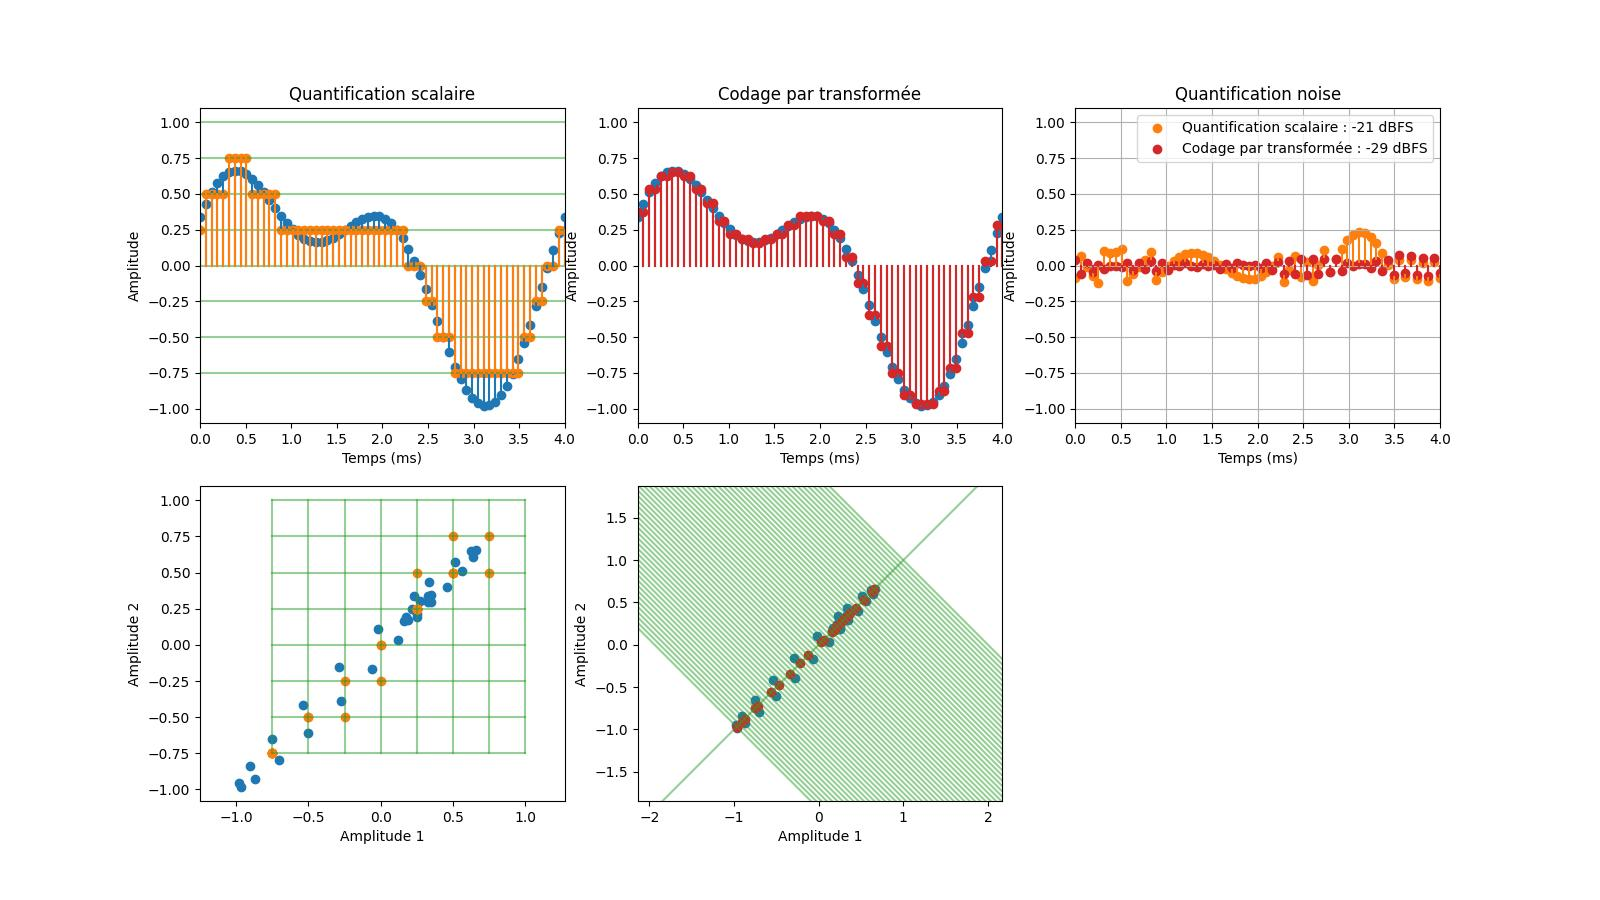
\includegraphics[width=.8\textwidth]{fig/tc_example_8.jpg}}

\end{frame}

\begin{frame}{Codage par transformée : exemple réel sur de la parole} %-----------------------------------------------------

\animategraphics[loop,controls,width=.8\textwidth]{10}{fig/tc_speech_anime/tc_speech_}{1}{99}


\end{frame}



\begin{frame}{Quoi perdre ?} %-----------------------------------------------------
\begin{columns}
   \begin{column}{0.6\textwidth}
	
  \begin{itemize}
  	\item Idée : s'appuyer sur les faiblesses de nos sens
  	\item Exemple (visuel) :
  	\begin{itemize}
      \item On est plus sensible à la luminosité que la couleur
      \item On entend pas un son faible proche d'un son fort  	
  	\end{itemize}

  \end{itemize}
   \end{column}
   \begin{column}{0.39\textwidth}
		
   \end{column}
\end{columns}
\end{frame}

\begin{frame}[allowframebreaks]{Sous-échantillonnage des couleurs} %-----------------------------------------------------
\begin{columns}
   \begin{column}{0.6\textwidth}
    RVB $\rightarrow$ Luminance-chrominanceB-chrominanceR
   \end{column}
   \begin{column}{0.39\textwidth}
		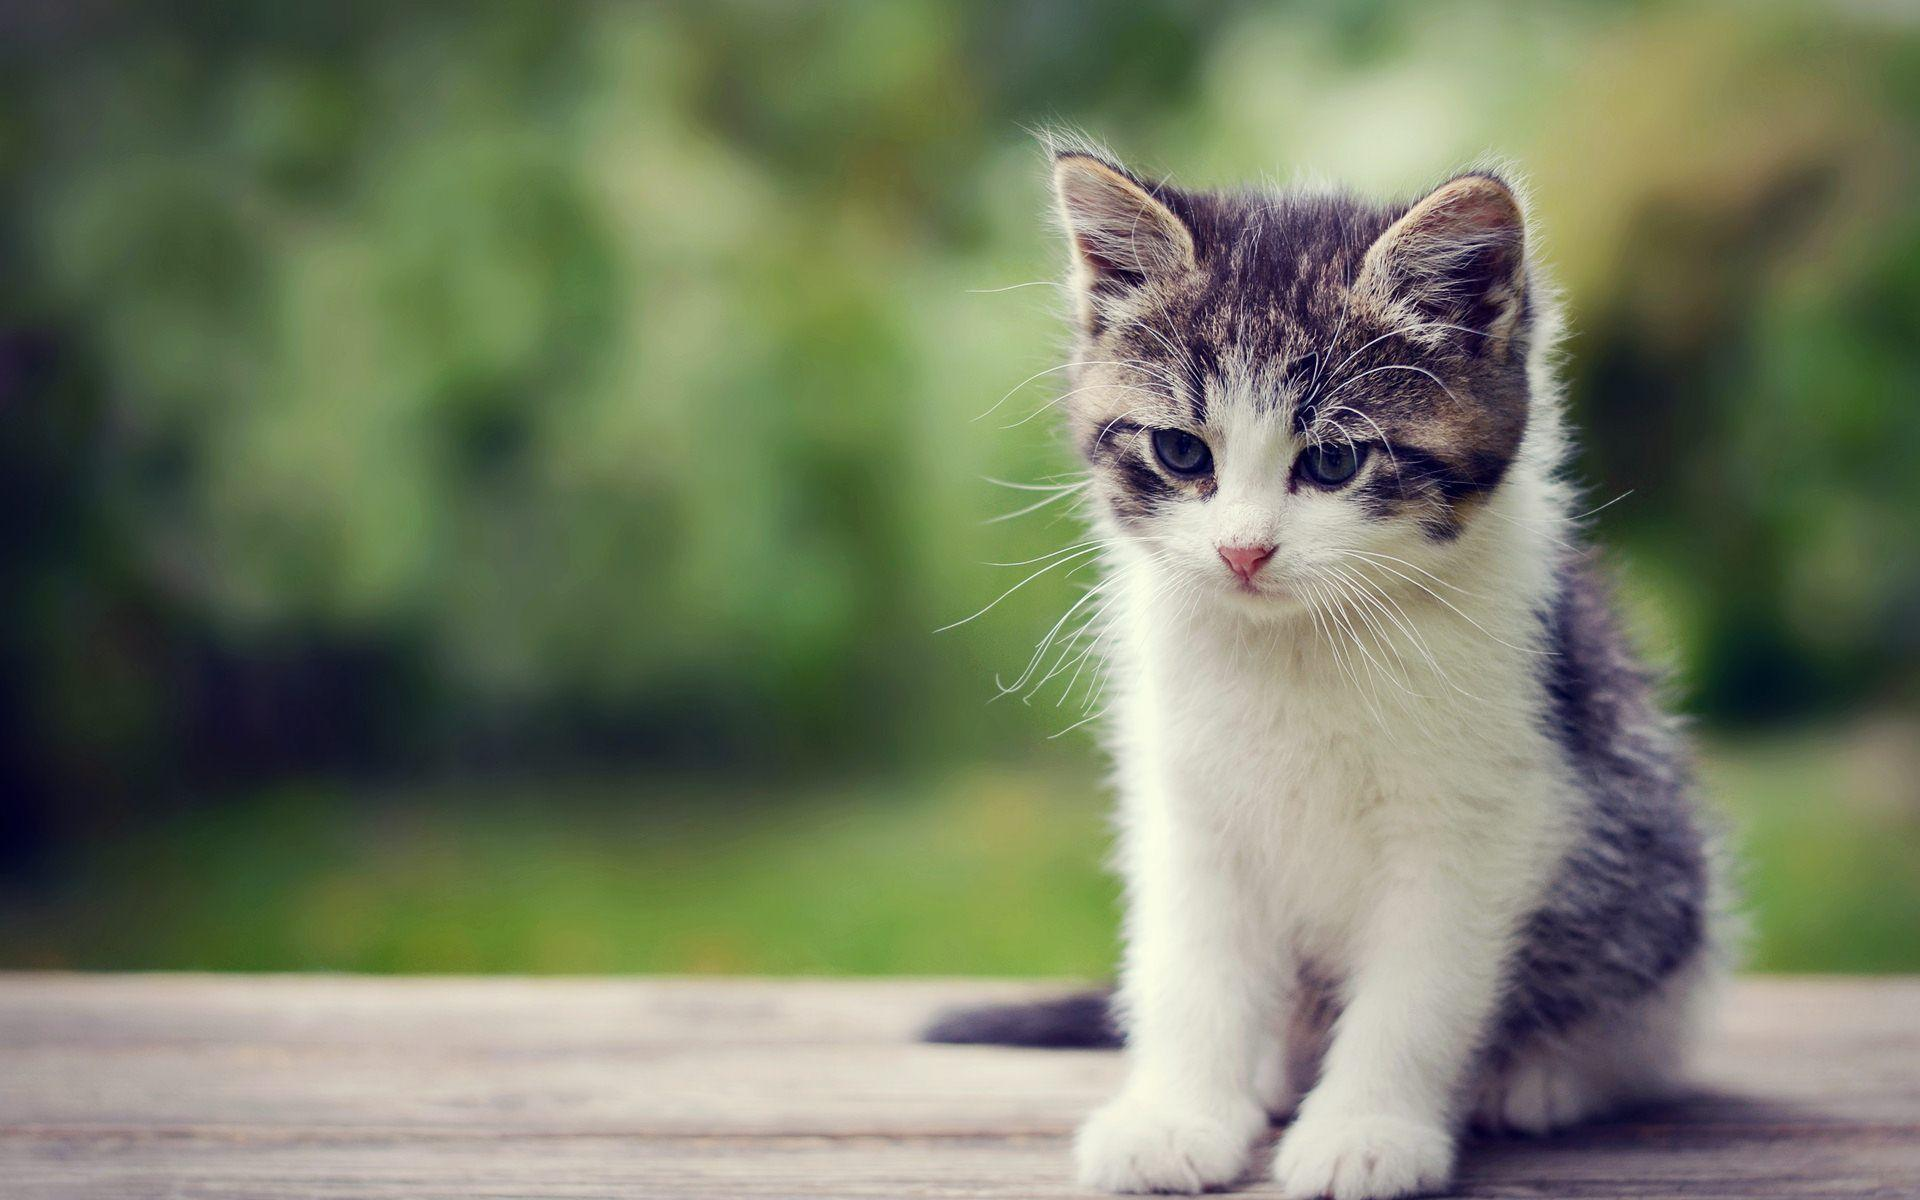
\includegraphics[width=\textwidth]{fig/cat/cat.jpg}
        
   \end{column}
\end{columns}
\framebreak
\animategraphics[loop,controls,width=.8\textwidth, trim=100 50 100 50, clip]{10}{fig/cat/cat_rgb_yuv/img_}{1}{59}
\end{frame}

\begin{frame}{Codage par transformée : changer de point de vue} %-----------------------------------------------------
\begin{columns}
   \begin{column}{0.6\textwidth}
		Applications :
        \begin{itemize}
            \item Image : JPEG
            \item Audio : MP3, AAC
        \end{itemize}

   \end{column}
   \begin{column}{0.39\textwidth}
		
   \end{column}
\end{columns}
\end{frame}

%==================================================================================================
%==================================================================================================
%==================================================================================================	
\section{Compression neuronale}

\begin{frame}{} %-----------------------------------------------------
\begin{center}
\Huge \insertsection
\end{center}
\end{frame}

\begin{frame}{Réseau de neurones : approximateur de fonction} %-----------------------------------------------------
\begin{columns}
   \begin{column}{0.48\textwidth}
		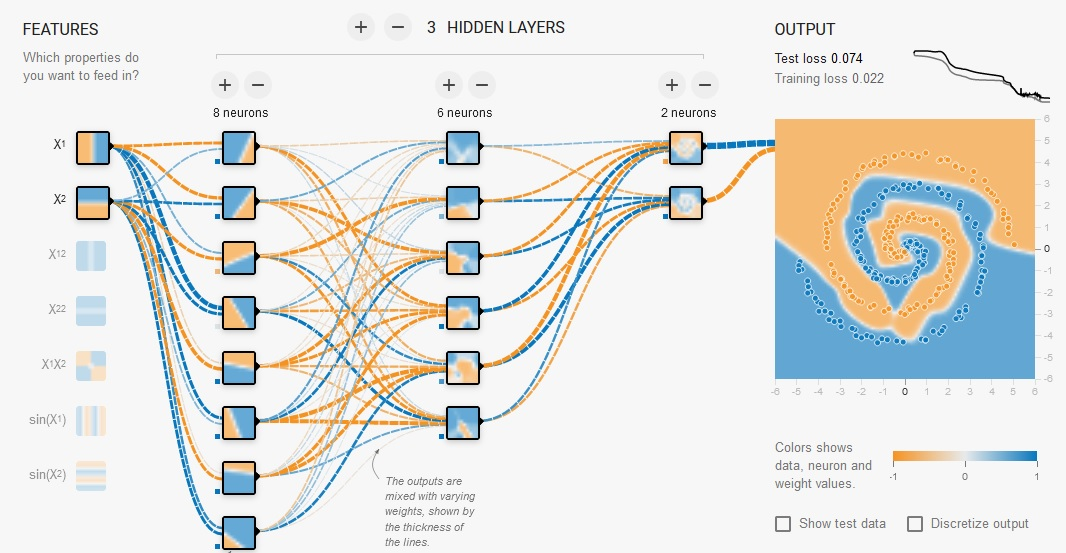
\includegraphics[width=\textwidth]{fig/deeperplayground.jpg}
   \end{column}
   \begin{column}{0.48\textwidth}
		%
   \end{column}
\end{columns}
\url{https://deeperplayground.org/}
\end{frame}

\begin{frame}{Réseau de neurones auto-encodeur} %-----------------------------------------------------
\begin{columns}
   \begin{column}{0.48\textwidth}
		%
   \end{column}
   \begin{column}{0.48\textwidth}
		%
   \end{column}
\end{columns}
\end{frame}

\begin{frame}{Réseau de neurones auto-encodeur} %-----------------------------------------------------
\begin{columns}
   \begin{column}{0.48\textwidth}
		%
   \end{column}
   \begin{column}{0.48\textwidth}
		%
   \end{column}
\end{columns}
\end{frame}

%==================================================================================================
%==================================================================================================
%==================================================================================================	
\section{Résumé}

\begin{frame}{} %-----------------------------------------------------
\begin{center}
\Huge \insertsection
\end{center}
\end{frame}

\begin{frame}{Compression sans pertes : codage entropique} %-----------------------------------------------------
\begin{columns}
   \begin{column}{0.48\textwidth}
		%
   \end{column}
   \begin{column}{0.48\textwidth}
		%
   \end{column}
\end{columns}
\end{frame}

\begin{frame}{Compression avec pertes} %-----------------------------------------------------
\begin{columns}
   \begin{column}{0.48\textwidth}
		%
   \end{column}
   \begin{column}{0.48\textwidth}
		%
   \end{column}
\end{columns}
\end{frame}

\begin{frame}{Compression neuronale} %-----------------------------------------------------
\begin{columns}
   \begin{column}{0.48\textwidth}
		%
   \end{column}
   \begin{column}{0.48\textwidth}
		%
   \end{column}
\end{columns}
\end{frame}

%==================================================================================================
%==================================================================================================
%======================================= TEMPLATE =================================================

%\begin{frame}{} %-----------------------------------------------------
%\end{frame}
%
%\begin{frame}{} %-----------------------------------------------------
%\begin{columns}
%    \begin{column}{0.48\textwidth}
%		%
%    \end{column}
%    \begin{column}{0.48\textwidth}
%		%
%    \end{column}
%\end{columns}
%\end{frame}

\end{document}